\section{Применение эволюционных алгоритмов для настройки гиперпараметров.}

\subsection*{Абстрактная оптимизация}

Можно вычислять функцию ошибки на любом входе.

Применяется для медленных, невыпуклых, недифференцируемых
функций.

Критерии остановки:
\begin{itemize}
    \item Число вызовов оптимизируемой функции
    \item Время работы
    \item Требуемое значение функции
\end{itemize}

Операторы для работы с абстрактным пространством:
\begin{itemize}
    \item Генерация = выдает новый объект
    \item Мутация = делает новый объект, похожий на старый
    \item Кроссовер = делает из двух объектов третий, похожий
    на родителе
\end{itemize}

Случайный поиск = n запусков оператора генерации.

\begin{algorithm}[H]
\caption{Hill climbing}
$x \gets rand()$

\While{$StoppingCriteria() = false$}{
    $x' \gets mutate(x)$

    \If{$L(x') < L(x)$}{
        $x \gets x'$
    }
}
\end{algorithm}

Можно запускать несколько раз из разных точек, чтобы не падать
в локальный минимум.

\begin{algorithm}[H]
    \caption{Имитация отжига}
    $x \gets rand(), t \gets T_start$

    \While{$StoppingCriteria()$ = false}{
        $x' \gets mutate(x)$

        \If{$random() < exp((L(x) - L(x')) / t)$}{
            $x \gets x'$
        }

        $t \gets decrease(t)$
    }
\end{algorithm}

Полноценный генетический алгоритм также использует оператор
кроссовера и оператор селекции, выбирающий элементы из популяции
для скрещивания.

\subsection*{Численные методы}

\subsubsection*{Субградиентные методы}

\begin{itemize}
    \item Аппроксимируем производную
    
    $\frac{\partial L}{\partial x_j} =
    \frac{L(x + \delta onehot(j)) - L(x)}{\delta}$
    \item Минимизируем градиентным спуском
    
    $x_{new} = x_{old} - \lambda \frac{\partial L}{\partial x}$
\end{itemize}


\subsubsection*{Дифференциальная эволюция}

\begin{itemize}
    \item Выберем $a, b, c: L(a) < L(b)$
    \item Добавим в популяцию $d = c + (b - a)$
    \item Удалим из популяции худший объект
\end{itemize}

*Двигаем c к лучшему будущему.

\subsubsection*{Метод Роя Частиц}

\begin{algorithm}
    $[x_i] \gets current\ coords$

    $[v_i] \gets current\ velocity$

    $[b_i] \gets best\ historical\ coords\ for\ each\ obj$

    $g \gets \arg \max_{b_i} L(b_i)$

    $\omega, \phi_b, \phi_g \gets consts$

    \For{$n$}{
        \ForEach{$x \in [x_i]$}{
            \ForEach{$j \in coords$}{
                $r_b, r_g \gets rand(0, 1)$

                $v_{ij} \gets \omega v_{ij} +
                \phi_b r_b (b_{ij} - x_{ij}) +
                \phi_g r_g (g - x_{ij})$
            }
            $x_i \gets x_i + v_i$

            $b_i \gets \arg \min_{x \cap b_i} L(x)$

            $g \gets \arg \min_{b \cap g} L(x)$
        }
    }
\end{algorithm}

% \begin{figure}[H]
% 	\centering
% 	\begin{minipage}[b]{0.4\textwidth}
% 		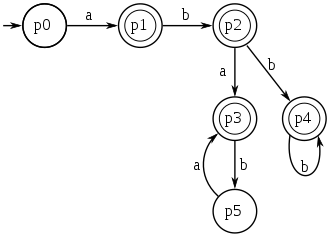
\includegraphics[width=\textwidth]{images/dfa.png}
% 		\caption{Пример графа переходов детерминированного КА.}
% 	\end{minipage}
% 	\hfill
% 	\begin{minipage}[b]{0.4\textwidth}
% 		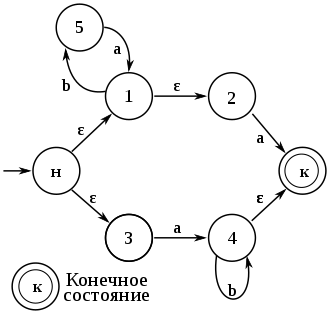
\includegraphics[width=\textwidth]{images/ndfa.png}
% 		\caption{Пример графа переходов недетерминированного КА с самопроизвольными переходами.}
% 	\end{minipage}
% \end{figure}